\section{Dioden}

\begin{tabular}{ll}
    Kleinsignal-Ersatzschaltung:    &  Kleinsignal-Widerstand $r_d$ \\
    Grosssignal-Ersatzschaltung:    & Spannungsquelle + $r_d$
\end{tabular}


\subsection{Aufbau}

\begin{minipage}[c]{0.4\columnwidth}
    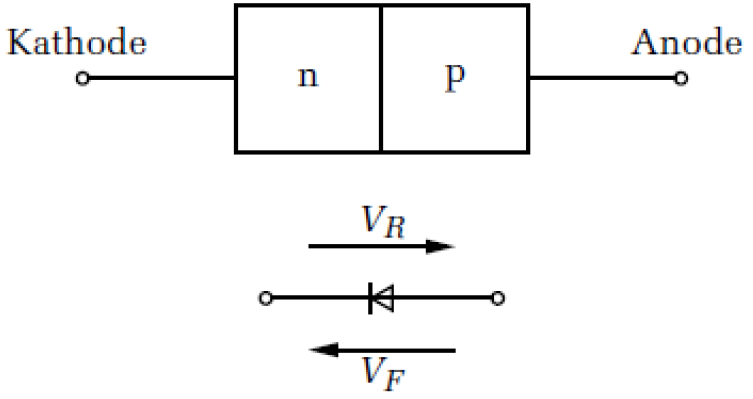
\includegraphics[width=\columnwidth]{images/diode.png}
\end{minipage}
\hfill
\begin{minipage}[c]{0.55\columnwidth}
    \raggedright
    Positiver Strom in Flussrichtung    \\
    (Anode \textrightarrow\ Kathode)

    \vspace{0.2cm}

    \textbf{Stromverdoppelung alle $\bm{20 \milli \volt}$}
\end{minipage}

\vspace{0.2cm}

\begin{minipage}[c]{0.3\columnwidth}
    \begin{center}
        Für $ V_d < 200 \, \milli \volt $
        $$ \boxed{ I_D = I_S \Big( e^{\frac{V_D}{n \cdot V_T}} -1 \Big)} $$
    \end{center}
\end{minipage}
\hfill
\begin{minipage}[c]{0.65\columnwidth}
    \begin{center}
        Für $ V_d > 200 \, \milli \volt $
        $$ \boxed{ I_D = I_S \cdot e^{\frac{V_D}{n \cdot V_T}}} \qquad \bm{V_T} = \frac{k_B \cdot T}{q} \bm{ \approx 25 \, \milli \volt} $$
    \end{center}
\end{minipage}

\vspace{0.3cm}

\begin{tabular}{ll}
    $I_S$   & Sättigungsstrom $(\pico \ampere \ldots \nano \ampere)$                        \\
    $n$     & Emissionskoeffizient $1 < n < 2$                                              \\
    $k_B$   & Boltzmann-Konstante $k_B = 1.38 \cdot 10^{-23} \, \frac{\joule}{\kelvin} $    \\
    $T$     & \textbf{Absolute} Temperatur in $\kelvin$
\end{tabular}


\subsection{Ersatzschaltungen}

\subsubsection{Grosssignal-Ersatzschaltung}

\begin{minipage}[c]{0.46\columnwidth}
    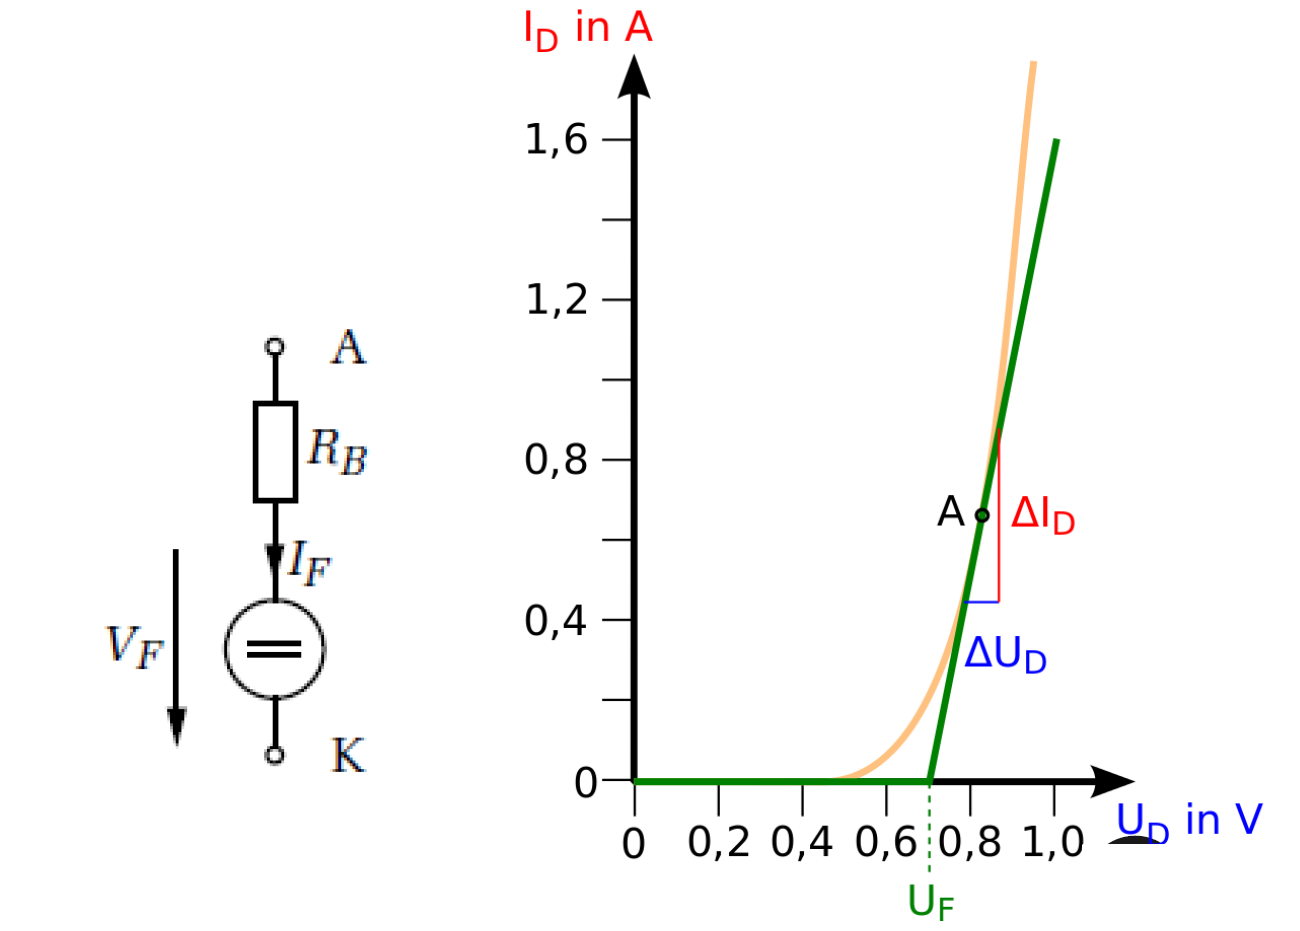
\includegraphics[width=\columnwidth]{images/vereinfachte_reale_diode.png}
\end{minipage}
\hfill
\begin{minipage}[c]{0.53\columnwidth}
    \myul{\textbf{Tangente im Arbeitspunkt}}

    \vspace{0.1cm}

    \begin{tabular}{ll}
        $r_d$:  & Steigung der Kennlinie \\
        $V_F$:  & Verlängerung Tangente  \\
                & (Schnittpunkt)
    \end{tabular}

    $$ \boxed{ g = \frac{1}{r_d} = \frac{\diff I_D}{\diff V_D} } $$
    $$ \boxed{ g = \frac{1}{n \cdot V_T} I_S \cdot e^{\frac{V_D}{n \cdot V_T}} = \frac{I}{n \cdot V_T} } $$
\end{minipage}


\subsubsection{Kleinsignalersatzschaltung}

Nur Widerstand $r_d$ \textbf{ohne Spannungsquelle}

\vspace{0.1cm}

\begin{tabular}{ll}
    Diode sperrt:   & $r_d = \infty$            \\
    Diode leitet:   & $r_d$ gemäss Kennlinie
\end{tabular}


\subsection{Temperaturverhalten}

\begin{minipage}[c]{0.35\columnwidth}
    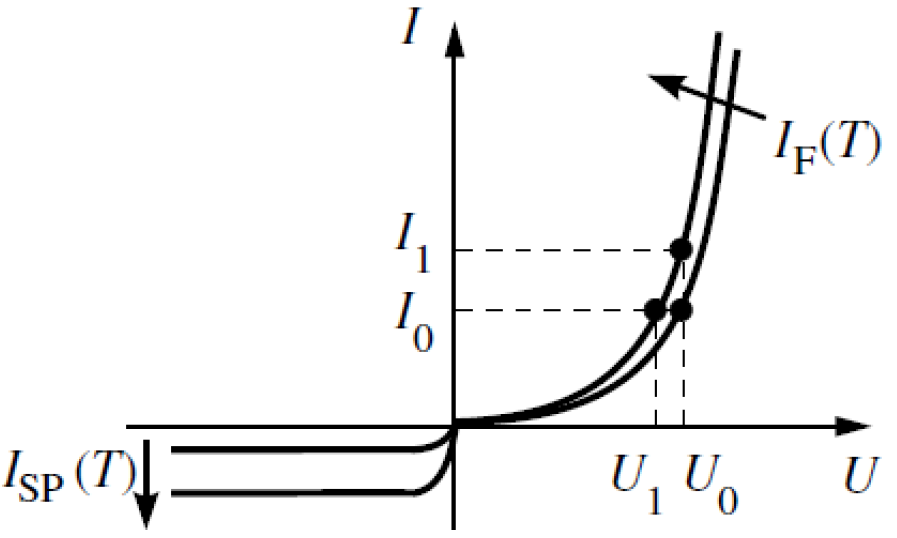
\includegraphics[width=\columnwidth]{images/diode_temperaturverhalten.png}
\end{minipage}
\hfill
\begin{minipage}[c]{0.62\columnwidth}
    \raggedright
    \myul{\textbf{Leitender Bereich}}

    \vspace{0.1cm}

    $$ \boxed{ \frac{\diff V_F}{\diff T} = -2 \, \frac{\milli \volt}{\kelvin} \quad \text{@ }  I = \const } $$

    \vspace{0.1cm}

    \textbf{ \textrightarrow\ Diodenspannung nimmt pro $\bm{\celsius}$ um $\bm{2 \, \milli \volt}$ ab}
\end{minipage}

\vspace{0.2cm}

\myul{\textbf{Sperrender Bereich}}

\vspace{0.1cm}

\begin{itemize}
    \item Sperrstrom-Zunahme erfolgt exponentiell mit der Temperatur
    \item Verdoppelung des Sperrstroms bei Temperatur-Erhöhung um $10 \, \celsius$ \\
        \textrightarrow\ Verdoppelung der Ausfallrate!
\end{itemize}


\subsubsection{Thermische Spezifikation}

\begin{itemize}
    \item \textbf{Temperatur von Silizium-Halbleitern darf $\bm{170 \celsius}$ nicht überschreiten}
    \item Bauform (Gehäuse) wird abhängig vom max. Strom bzw. der zulässigen Verlustleistung gewählt
    \item Mit grösserer Siliziumfläche erhöht sich auch der Sättigungssperrstrom $I_S$
    \item Thermischer Widerstand $R_{\theta}$ in $\celsius / \watt$ gibt an, wieviel sich Halbleiter mit Verlustleistung erwärmt 
\end{itemize}


\subsection{Dioden bei negativer Spannung}

\begin{minipage}[c]{0.35\columnwidth}
    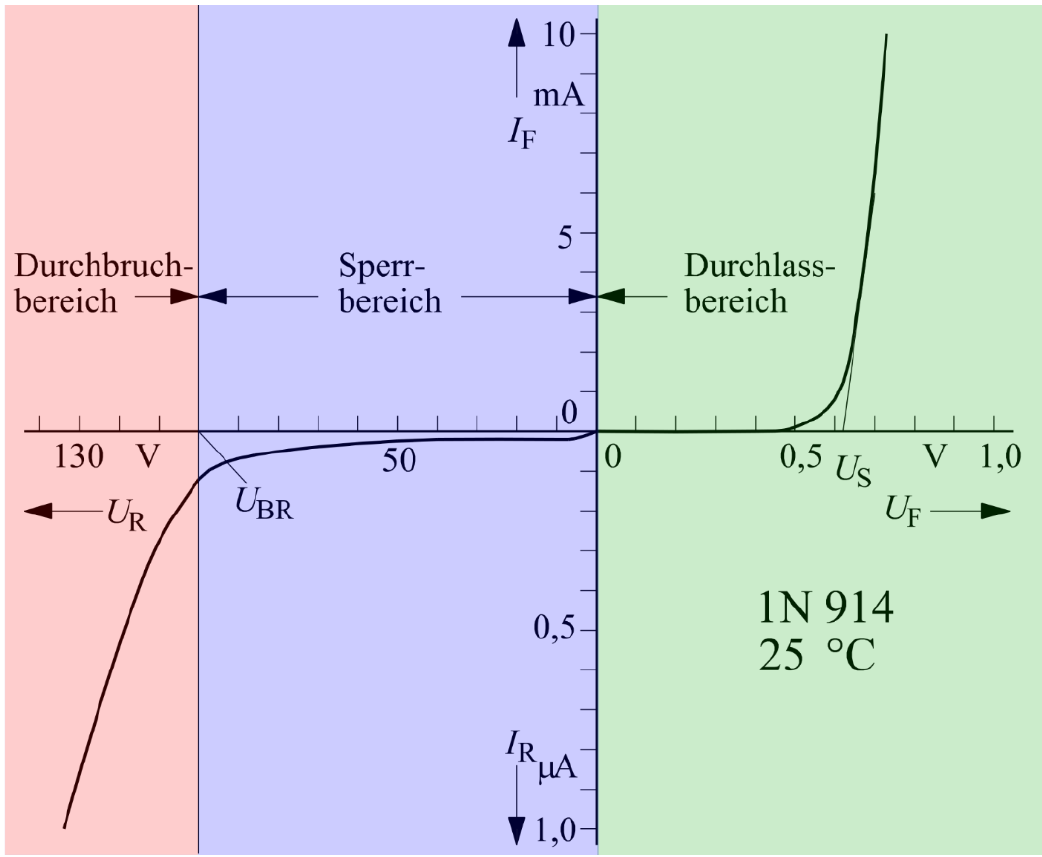
\includegraphics[width=\columnwidth]{images/diodenbereiche.png}
\end{minipage}
\hfill
\begin{minipage}[c]{0.62\columnwidth}
    \textbf{Diodendurchbruch @ $\bm{V_{\rm BR}$}}

    \vspace{0.1cm}

    Bei hoher negativer Sperrspannung steigt Sperrstrom zunächst langsam und dann schlagartig an. \\
    Gleichrichterdioden: $V_{\rm BR} \approx 50 \, \volt \, \ldots \, 1000 \, \volt $
\end{minipage}


\subsection{Diodenschaltungen}

\subsubsection{Diode mit Seriewiderstand}


\begin{minipage}[c]{0.4\columnwidth}
    \begin{center}
        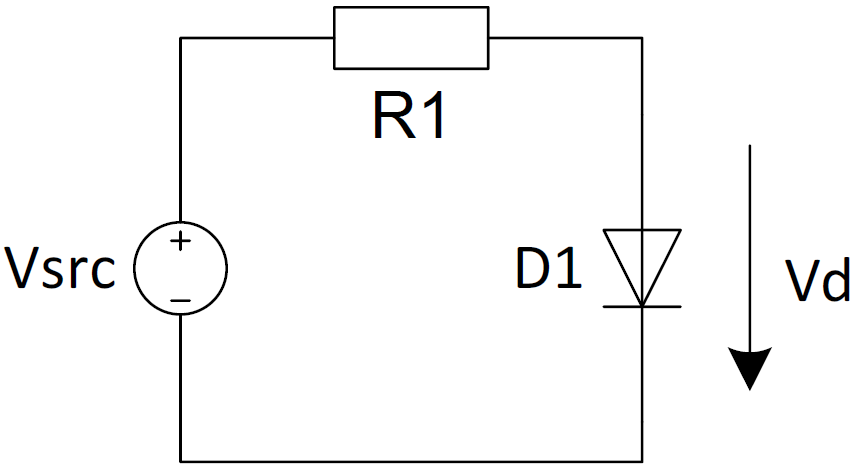
\includegraphics[width=0.8\columnwidth]{images/diode_mit_seriewiderstand.png}

        \vspace{0.2cm}

        \cbl{\textbf{Widerstandsgerade:} }
        $$I_{KS} = \frac{V_{SRC}}{R_1} \quad  (\text{@ } V_d = 0) $$
        $$ U_0 = V_{\rm SRC} \quad (\text{@ } I = 0) $$
    \end{center}
\end{minipage}
\hfill
\begin{minipage}[c]{0.5\columnwidth}
    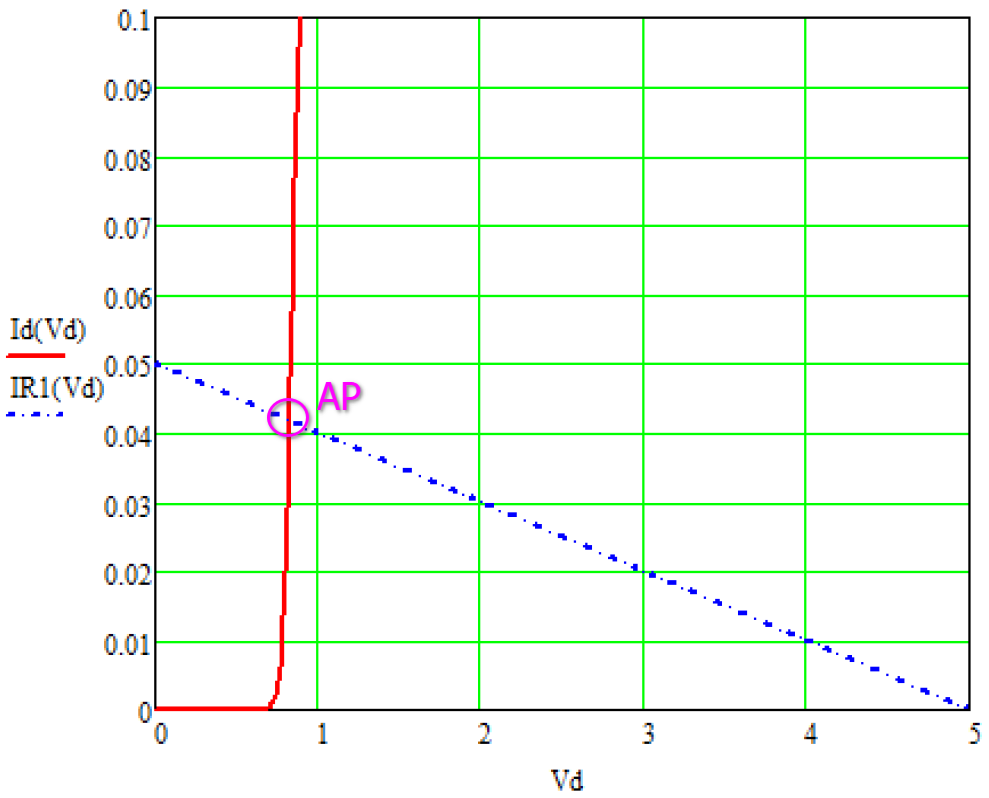
\includegraphics[width=\columnwidth]{images/diode_mit_seriewiderstand_kennlinie.png}
\end{minipage}


\subsubsection{Einweg-Gleichrichter}

\begin{minipage}[c]{0.35\columnwidth}
    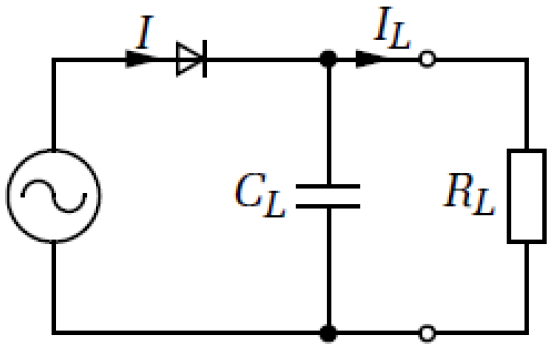
\includegraphics[width=\columnwidth]{images/einweggleichrichter.png}
\end{minipage}
\hfill
\begin{minipage}[c]{0.6\columnwidth}
    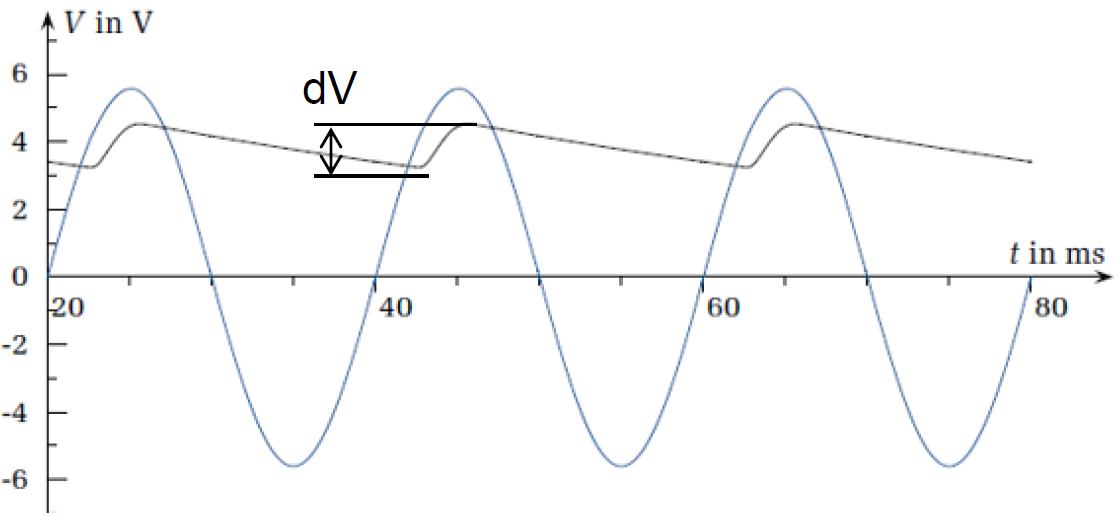
\includegraphics[width=\columnwidth]{images/einweggleichrichter_spannung.png}
\end{minipage}

\vspace{0.2cm}

\begin{minipage}[c]{0.52\columnwidth}
    \begin{tabular}{@{}ll@{}}
        Diode leitet:   & $V_{\rm out}= V_{\rm in} - V_D$               \\
        Diode sperrt:   & $V_{\rm out}= 0 \, \volt$                     \\
        Entladen:       & $C$ wird über $R$ entladen                    \\
                        & $V_{\rm out}(t) = e^{- \frac{t}{R \cdot C} }$ \\
        Rippelspannung: & $\diff V$                                     \\
        Laststrom:      & $I_0 = \frac{V_{\rm in}}{R_L}$
    \end{tabular}
\end{minipage}
\hfill
\begin{minipage}[c]{0.4\columnwidth}
    \raggedright
    Je kleiner die Rippel-Spannung,

    \vspace{0.1cm}

    \begin{itemize}
        \item desto kürzer die Aufladezeit
        \item desto grösser der maximale Strom
    \end{itemize}
\end{minipage}


\subsubsection{Brücken- / Vollwellengleichrichter}

\begin{minipage}[c]{0.45\columnwidth}
    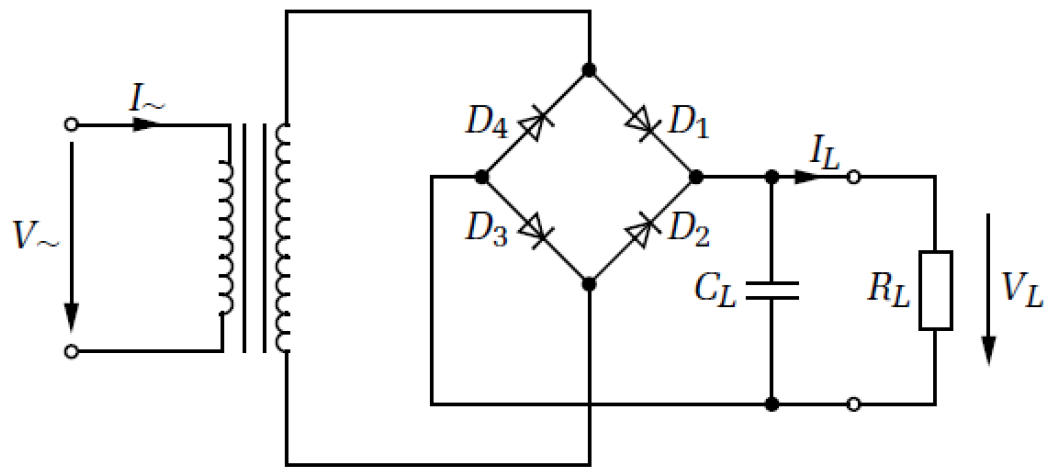
\includegraphics[width=\columnwidth]{images/brueckengleichrichter.png}
\end{minipage}
\hfill
\begin{minipage}[c]{0.52\columnwidth}
    \begin{itemize}
        \item[+] Nur halbe Rippel-Spannung
        \item[+] symm. Netzbelastung
        \item[-] Doppelter Spannungsverlust (2 Dioden)
    \end{itemize}
\end{minipage}



\subsection{Spannungsvervielfacher}

\subsubsection{Dickson Charge Pump $\bm{(N = 2)}$}

\begin{minipage}[c]{0.5\columnwidth}
    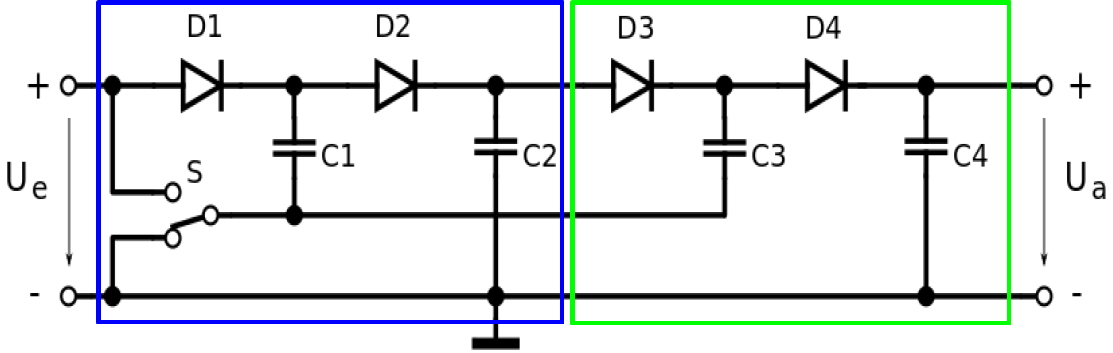
\includegraphics[width=\columnwidth]{images/dickson_charge_pump.png} 
\end{minipage}
\hfill
\begin{minipage}[c]{0.48\columnwidth}
    Aus kleiner DC-Spannung wird grössere DC-Spannung erzeugt 
    $$ \boxed{ U_a = (N+1) \cdot U_e - N \cdot 2 \cdot U_D} $$
\end{minipage}


\subsubsection{Villard-Schaltung (Spannungsverdoppler)}

\begin{minipage}[c]{0.4\columnwidth}
    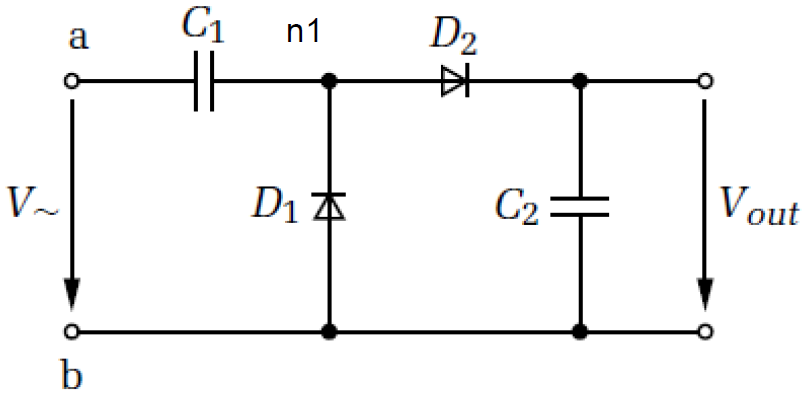
\includegraphics[width=\columnwidth]{images/villard_schaltung.png}
\end{minipage}
\hfill
\begin{minipage}[c]{0.58\columnwidth}
    $$ \boxed{ V_{\rm out} = 2 \cdot V_{\rm in} - 2 \cdot V_D} $$

    \begin{itemize}
        \item Verfielfacht AC-Spannungen
        \item $V_{\rm in} > 0$ Strom über $D_2$ in Last
        \item $V_{\rm in} < 0$ Strom über $D_1$ und $C_1$
        \item Spannung an $n1$ wird angehoben 
    \end{itemize}
\end{minipage}


\subsection{Spezielle Dioden}

\subsubsection{Schottky-Dioden}

\begin{minipage}[c]{0.3\columnwidth}
    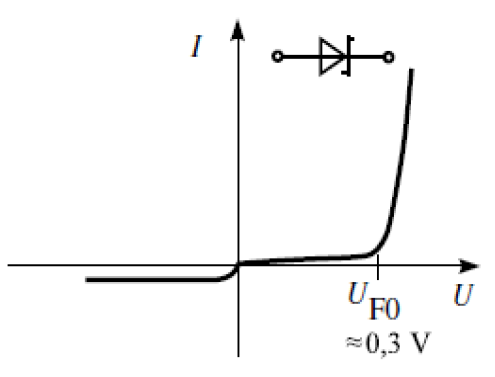
\includegraphics[width=\columnwidth]{images/schottky_diode.png}
\end{minipage}
\hfill
\begin{minipage}[c]{0.68\columnwidth}
    \raggedright
    
    \begin{itemize}
        \item \textbf{Flussspannung:} $ \bm{V_{\rm F0} \approx 0.3 \, \volt}$
        \item Viel höherer Sättigungs-Sperrstrom als Si-Diode \\
            \textrightarrow\ Für kleine Ströme ok
        \item Stromanstieg weniger steil als bei Si-Diode 
        \item Grössere Leckströme
    \end{itemize}
\end{minipage}


\subsubsection{Zener-Dioden / Z-Dioden}

\begin{minipage}[c]{0.4\columnwidth}
    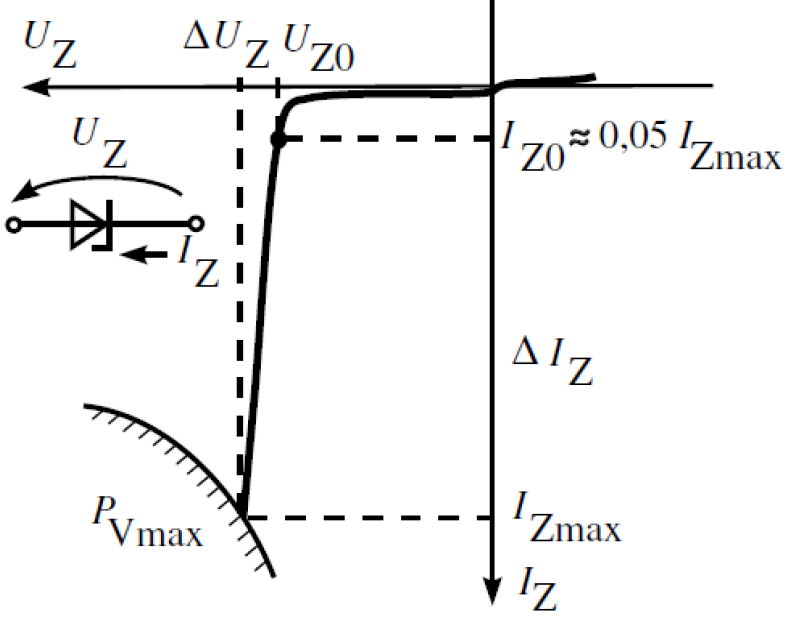
\includegraphics[width=\columnwidth]{images/zener_diode.png}
\end{minipage}
\hfill
\begin{minipage}[c]{0.45\columnwidth}
    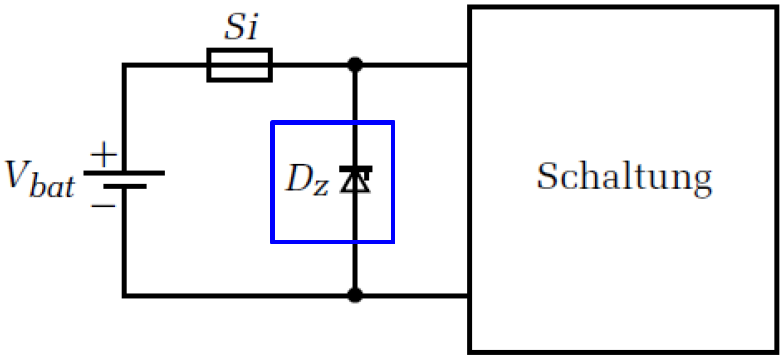
\includegraphics[width=\columnwidth]{images/anwendung_zener_diode.png}
\end{minipage}

\vspace{0.2cm}

\begin{itemize}
    \item \textbf{Anwednung im Durchbruchbereich}
    \item Eingesetzt als Spannungsbegrenzer / Spannungsreferenz \\
        \textrightarrow\ Z-Diode limitiert Spanung am Eingang der Schaltung 
    \item Temperatur-stabilste Referenzspannung $\bm{V_z = 5.6 \, \volt}$
\end{itemize}


\subsubsection{Germanium-Dioden}

\begin{itemize}
    \item Sehr kleine Schwellspannung: $V_D = 0.1 \, \ldots \, 0.4 \, \volt$
    \item Tiefe Temperaturzulässsigkeit: $T_{\rm max} = 75 \, \celsius$ \\
        \textrightarrow\ maximale Stromdichte wesentlich grösser als bei Si-Dioden
\end{itemize}


\subsubsection{Kapazitäts-Diode (Varicap)}

\begin{minipage}[c]{0.45\columnwidth}
    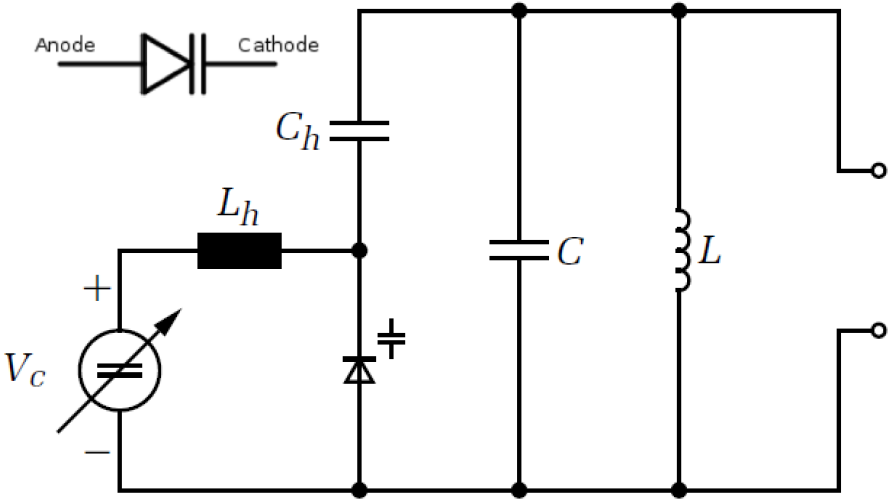
\includegraphics[width=\columnwidth]{images/kapazitaetsdiode.png}
\end{minipage}
\hfill
\begin{minipage}[c]{0.52\columnwidth}
    \raggedright

    \begin{itemize}
        \item Diode mit speziell grosser Kapazität \\
            \textrightarrow\ $C$ sinkt mit steigender Spannung 
        \item Einstellen der Schwingfrequenz in Oszillatoren 
    \end{itemize}
\end{minipage}

